\chapter{Cadena de simulaciones y an\'alisis de datos}

% En el proyecto Auger diversos grupos trabajan paralelamente en las diferentes fases del proyecto.
% En su mayor\'ia, estos grupos requieren simular tanto las lluvias como la respuesta del detector.
% Por este motivo, es importante fijar un marco de desarrollo que permita el intercambio de código dentro de la colaboraci\'on y asegure la compatibilidad entre programas. 

Dada la complejidad del problema, la \'unica manera viable de estimar la exposici\'on del detector al flujo de neutrinos es mediante simulaciones.
Para ello, son necesarios una serie de programas que se encargan de simular las distintas etapas del proceso de detecci\'on, ya descriptas en el cap\'itulo \ref{ch:deteccion}.
En la figura \ref{fig:sim_chain} se se\~nala qu\'e programa de simulaci\'on se utiliza en cada una de estas etapas.
%
\begin{figure}[h!]
	\begin{center}
	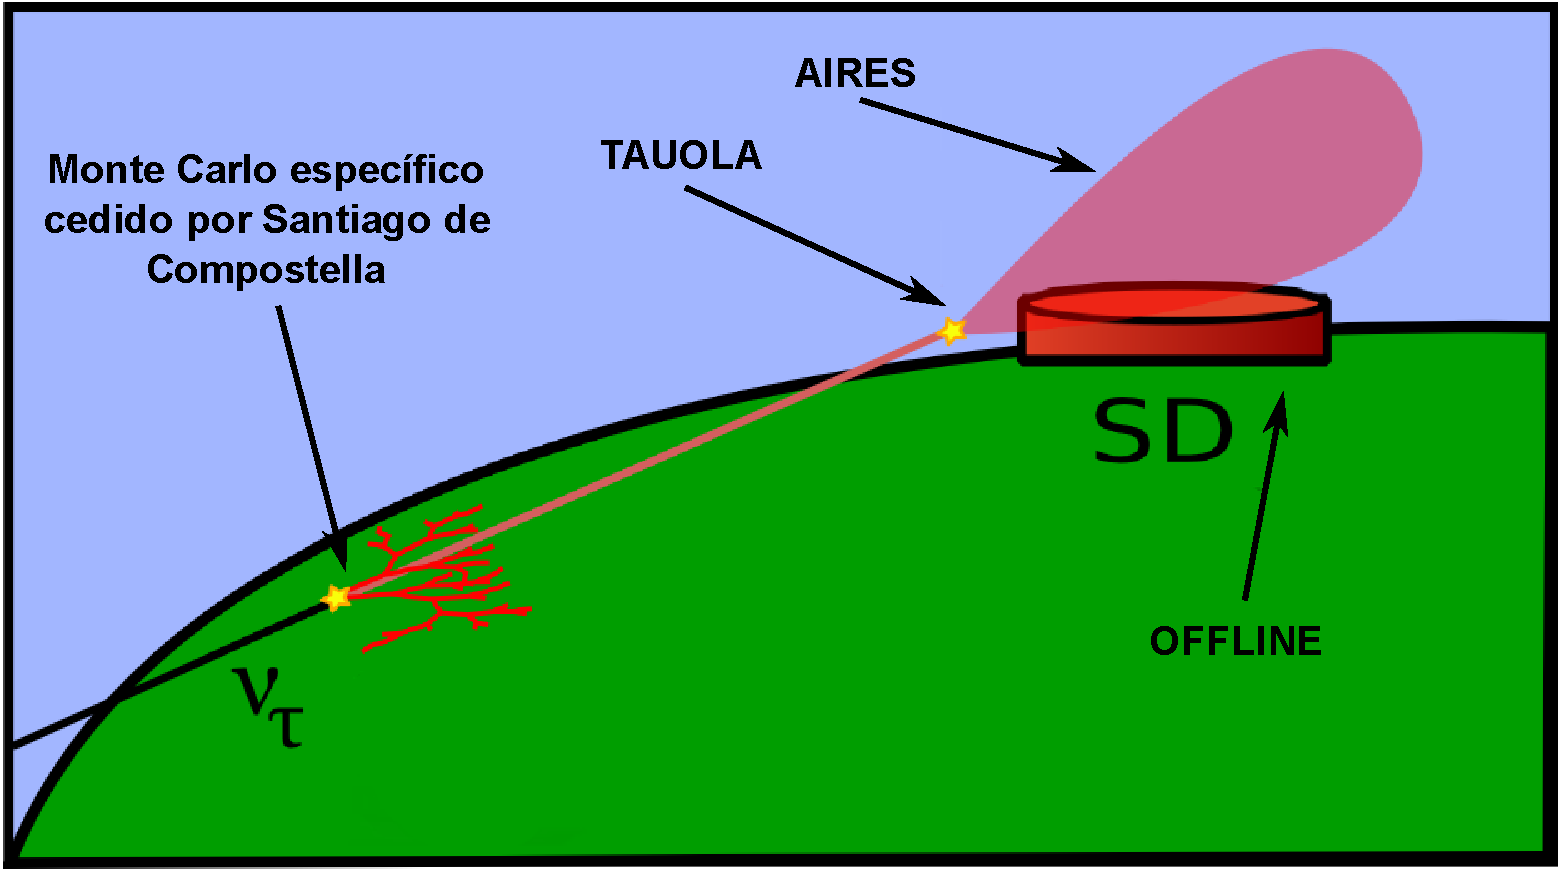
\includegraphics[width=0.75\textwidth]{fig/simulacionAuger/sim_chain}
	\caption{\label{fig:sim_chain} Se se\~nalan los programas utilizados para simular cada etapa del proceso de detecci\'on de los neutrinos rasantes.}
	\end{center}
\end{figure}
%

	\section{\label{sc:sim_prop_tierra}Propagaci\'on dentro de la tierra}
	
	Para simular la propagaci\'on del \tauon{} en la tierra se utiliz\'o un programa que realiza el c\'alculo mediante m\'etodos de Monte Carlo, desarrollado por J. A. Mu\~niz y E. Zas, del grupo de altas energ\'ias de la Universidad de Santiago de Compostela.
	Una explicaci\'on detallada del programa puede encontrarse en \cite{gap_tau_tierra}.
	
	Este c\'odigo permite propagar los \nutau{}s y \tauon{}s en la tierra y, dado el \'angulo cenital \tita{} y la energ\'ia del neutrino incidente \enu{}, calcular la probabilidad de que un \tauon{} alcance la superficie de la tierra con energ\'ia \etau{}.
	Estos c\'alculos se realizan teniendo en cuenta la interacci\'on del \nutau{} via CC y CN, la p\'erdida de energ\'ia del \tauon{} (con $\beta$\footnote{ver ecuaci\'on \ref{eq:tau_losses}} dependiente o independiente de la energ\'ia) y la regeneraci\'on del flujo de \nutau{} debido a interacciones via CN y a decaimientos de leptones \tauon{}.
	
	La simulaci\'on consta de dos etapas principales que se alternan hasta que se alcanza la superficie:
	
	\begin{description}
	\item[\textbf{Interacci\'on del \nutau{}:}] Se hace interactuar al neutrino siguiendo una distribuci\'on exponencial en $x$, donde $x$ es la variable que mide la cantidad de materia atravesada por el \nutau{}. Para ello, se tienen en cuenta interacciones via CC y CN. Si se diera una interacci\'on via CC, se produce un \tauon{} cuya energ\'ia proviene de muestrear la seccion efic\'az diferencial de CC, $\frac{d\sigma^{cc}}{dy}$. En cambio, si la interacci\'on se produce via CN, es generado un nuevo \nutau{} de energ\'ia menor que se hace interactuar nuevamente.
	\item[\textbf{Propagaci\'on del \tauon{}:}] En caso de que un \tauon{} sea producido, se lo propaga de a peque\~nos pasos, calculando en cada uno de ellos la energ\'ia perdida debido a la interacci\'on con el medio y la probabilidad de decaimiento (como funci\'on de su energ\'ia). Si decayese produciendo un nuevo \nutau{}, se comienza el procedimiento nuevamente desde el punto del \'ultimo decaimiento.
	\end{description}
	
	Este Programa fue validado utilizando programas mucho m\'as complejos, como ANIS \cite{anis}.
	Tambi\'en se realiz\'o una comparaci\'on del flujo de \tauon{} saliente obtenido mediante el calculo te\'orico que puede encontrarse en \cite{prop_tau} y el obtenido por este programa, para diferentes \'angulos cenitales.
	Esta \'ultima comparaci\'on se muestra en la figura \ref{fig:comp_tau_mc_teo}, en la que se observa un muy buen acuerdo entre ambos resultados.
	%
	\begin{figure}[h!]
		\begin{center}
		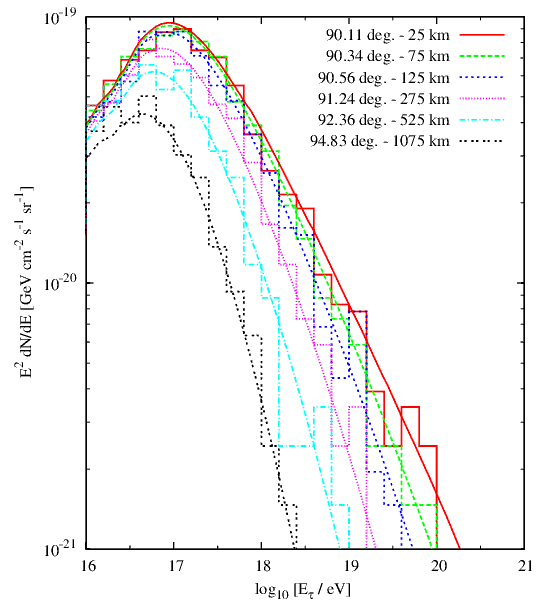
\includegraphics[width=0.75\textwidth]{fig/simulacionAuger/comp_tau_mc_teo}
		\caption{\label{fig:comp_tau_mc_teo} Comparaci\'on de los flujos salientes obtenido anal\'iticamente y mediante simulaci\'on. Los histogramas corresponden a los resultados del Monte Carlo, mientras que la l\'inea llena al c\'alculo te\'orico.}
		\end{center}
	\end{figure}
	%
	
	\section{Decaimiento del \tauon{}: \tauola{}}
	
	Luego de propagarse a trav\'es de la atm\'osfera, el \tauon{} decae generando una gran variedad de part\'iculas secundarias que luego inician la EAS.
% 	Si bien la probabilidad de decaimiento a los diferentes canales puede calcularse anal\'iticamente, existe de una manera pr\'actica y casi autom\'atica utilizando \tauola{}.
% 	
	Para generar eventos utilizando la probabilidad de decaimiento a cada canal pueden utilizarse un conjunto de librer\'ias llamadas \tauola{}.
	Estas consisten en varios programas Monte Carlo que implementan decaimientos lept\'onicos y semilept\'onicos.
	Como salida se entrega la topolog\'ia completa del evento, incluyendo neutrinos, resonancias intermedias y la estructura completa de spin durante el desarrollo del decaimiento.
	
	Como paquete universal para calcular decaimientos de leptones \tauon{}, \tauola{} cumple con los siguientes requerimientos:
	%
	\begin{itemize}
	\item El acoplamiento de \tauola{} a cualquier simulaci\'on Monte Carlo es simple.
	\item Se tienen en cuenta todos los efectos relacionados a la polarizaci\'on del \tauon{}, tanto en el decaimiento primario como en los decaimientos secundarios.
	\item La suma de probabilidades de todos los decaimientos del \tauon{} tenidos en cuenta suman pr\'acticamente el \cant{100}{\%}
	\item Los elementos de matr\'iz del decaimiento son accesibles y f\'acilmente modificables. Esto es muy pr\'actico si por ejemplo se quiere incluir nueva f\'isica.
	\end{itemize}
	
	Debido a todas estas ventajas, \tauola{} se utiliza muy frecuentemente dentro de la comunidad de altas energ\'ias.
	

	\section{Simulaci\'on de las EAS: Aires}

	En la actualidad existen varios programas para simular la formación de una EAS a partir de una partícula primaria a lo largo de la atmósfera terrestre.
	Entre ellos están {\sc corsika}, {\sc aires}, etc.
	En este trabajo se utilizaron EAS simuladas mediante {\sc aires}.

	{\sc Aires} es un conjunto de programas y subrutinas que simulan la lluvia de partículas luego de la incidencia de una rayo cósmico y permite administrar la información relacionada. 

	Este simulador provee un ambiente realista donde la propagación de las partículas se da teniendo en cuanta las características de la atmósfera, el campo geomagnético y la curvatura de la Tierra. 
	
	Debido a que la cantidad de part\'iculas generada en una EAS se vuelve rapidamente inmanejable\footnote{Por ejemplo, para una EAS cuya part\'icula primaria posee \cant{10^{17}}{eV} puede llegar a tener del orden de $10^8$ part\'iculas de energ\'ia mayor a \cant{100}{MeV}. Esto requerir\'ia de orden de \cant{100}{GB} para almacenarlas y 15 d\'ias de tiempo de m\'aquina para seguirlas a todas. Por lo general es necesario simular del orden de $10^3\textit{-}10^4$ EAS para hacer cualquier comparaci\'on con datos experimentales.
	}
	, es com\'un en estos programas utilizar un procedimiento estadístico de muestreo llamado {\em thinning}.
	Este consiste en tomar un \textit{set} representativo de part\'iculas que luego es propagado.
	La elecci\'on de dicho set es tal que no se alteran los valores medios de los observables de la lluvia.
	Una explicaci\'on del algoritmo puede encontrarse en \cite{thining}.

	Las partículas que se tienen en cuenta en las simulaciones son: gammas, electrones, positrones, muones, piones, kaones, mesones eta, bariones lambda, nucleones, antinucleones y núcleos de hasta Z=36.
	Los neutrinos electr\'onicos y mu\'onicos que son generados en ciertos decaimientos se tienen en cuenta en cuanto a la energía, pero no son propagados.
	
	La part\'icula que inicia la lluvia puede ser cualquiera de las mencionadas con energías que pueden variar en el rango de \cant{10^9{\it-}10^{21}}{eV}. 
	Tambi\'en es posible simular lluvias iniciadas por partículas primarias ``especiales'' utilizando un módulo que debe escribir cada usuario, capaz de procesar la primer interacción del primario y devolver una lista de part\'iculas tradicional que {\sc aires} pueda aceptar. 

	Los procesos físicos m\'as importantes (desde el punto de vista probabilístico) que las lluvias de part\'iculas pueden sufrir son tenidos en cuenta en las simulaciones. 
	Estos procesos son:

	\begin{itemize}
	\item Procesos electrodin\'amicos: producci\'on de pares y aniquilaciones electr\'on-positr\'on, bremsstrahlung (electrones, positrones y muones), producci\'on de pares mu\'onicos, electrones sacados de \'orbitas at\'omicas (rayos $\delta$), efectos Compton y fotoel\'ectrico, efecto Landau-Pomeranchuk-Migdal (LPM) y supresi\'on diel\'ectrica.
	\item Decaimientos de part\'iculas inestables.
	\item Procesos Hadr\'onicos: colisiones inel\'asticas hadr\'on-n\'ucleo y fot\'on-n\'ucleo, muchas veces simulados utilizando paquetes externos que implementan un modelo de interacci\'on hadr\'onico, como los modelos SIBYLL, QGSJET o QGSJET2, Reacciones fotonucleares, Fragmentaciones nucleares, elásticas e inelásticas.
	\item Propagaci\'on de part\'iculas cargadas: perdidas de energ\'ia en el medio (ionizaci\'on), dispersiones múltiples de Coulomb y deflexiones geomagn\'eticas.
	\end{itemize}    

	Tambi\'en, el sistema de simulación de {\sc aires} provee una plataforma que permite hacer uso del poder de c\'alculo de las computadoras actuales:
	
	\begin{itemize}
	\item Implementa un lenguaje de comandos iniciales (IDL por {\em Input Directive Language}), que consiste en un conjunto simple de comandos que permiten un control eficiente de los par\'ametros de entrada para cada simulación. 
	\item El sistema que lleva a cabo las simulaciones es una herramienta poderosa en plataformas UNIX, ya que permite al usuario coordinar muchas simulaciones en simultaneo, controlar la evolución de un dado trabajo mientras que se está llevando a cabo, etc.
	\item El programa que administra la información de salida procesa archivos generados por el programa principal y permite obtener información relacionada con los observables físicos durante y al final de cada simulación.
	\item Finalmente, hay una librería que provee una serie de rutinas auxiliares para procesar la información generada. En particular, la información m\'as relevante es contenida en archivos comprimidos. \'Esta consiste en informaci\'on detallada de cada part\'icula que llega al piso y de la lluvia en diferentes alturas, que se registra durante la evolución de la misma.
	\end{itemize}
	
	\section{Simulaci\'on del detector: Offline}
	
	Una vez la lluvia alcanza el nivel del suelo, es necesario simular la respuesta del detector, para lo que se utiliza \Offline{}.
	Este programa, desarrollado en C++, fue dise\~nado especialmente para cubrir los requerimentos del proyecto Auger. Por ejemplo:
	\begin{itemize}
	\item Contiene una intefaz intuitiva y f\'acil de comprender, que sigue la misma l\'ogica que el detector real.
	\item Dicha interfaz permite acceder a informaci\'on del detector u otros (archivada en diversos formatos) mediante comandos simples y estandarizados.
	\item Es posible cambiar completamente la implementaci\'on de cualquier algoritmo sin cambiar en absoluto la interfaz.
	\item Es posible simular un detector completamente heterog\'eneo en el que cada tanque o telescopio tiene identidad propia.
	\item El grado de detalle con el que se realizan las simulaciones puede variar f\'acilmente, seg\'un se necesite.
	\end{itemize}
	
	\subsection{Algoritmos dentro de Offline}
	
	Si bien \Offline{} posee una gran cantidad de algoritmos que se utilizan en diferentes \'areas dentro de la colaboraci\'on, aqu\'i s\'olo se introducen unos pocos que son importantes en este an\'alisis.
	
		\subsubsection{Unthinning}
		
		Una vez que la EAS alcanza el nivel del suelo, las part\'iculas presentes se guardan, por lo general, en archivos binarios en diversos formatos, que dependen del simulador empleado.
		Si se ha utilizado un algoritmo de thinning, cada part\'icula se guarda con un peso respectivo que hace referencia a la cantidad de part\'iculas que esta representa.
		\Offline{} no s\'olo permite leer archivos provenientes de varios simuladores (entre los que se encuentra {\sc Aires}), sino que tambi\'en aplica un algoritmo de \textit{unuhinning} de manera de regenerar las part\'iculas no simuladas y tenerlas en cuenta en la se\~nal sobre el detector.
		
		Dado que el \'area instrumentada a nivel del suelo es muy chica y s\'olo unas pocas de las part\'iculas que llegan a este nivel interactuan con el detector,
% 		Por este motivo, para realizar el \textit{unthinning}, 
		\Offline{} realiza el unthinning utilizando un \textit{m\'etodo de muestreo local}.
		Todas las part\'iculas dentro de cierta zona de muestreo (correspondiente a cada detector) son seleccionadas.
		Luego, se las dispersa espacial y temporalmente utilizando un m\'etodo estad\'istico, que se describe en \cite{unthinning1}.
		
		Una vez que las part\'iculas, clones de la primaria, son dispersadas se las inyecta en posiciones aleatorias de la pared del detector, teniendo en cuenta la direcci\'on de incidencia. 
		Un ejemplo de esto \'ultimo se muestra en la figura \ref{fig:unthinning_tank}.
		%
		\begin{figure}[h!]
			\begin{center}
			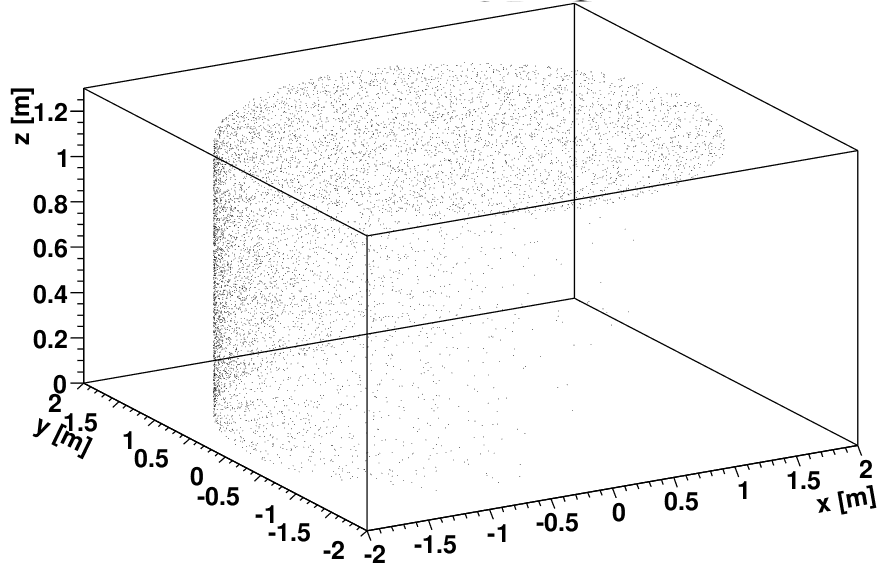
\includegraphics[width=0.7\textwidth]{fig/simulacionAuger/unthinning_tank}
			\caption{Distribuci\'on de part\'iculas sobre la superficie de un tanque luego de aplicar el algoritmo de unthinning.}
			\label{fig:unthinning_tank}
			\end{center}
		\end{figure}
		%
		
		En particular, el algoritmo de unthinning no es directamente aplicable a lluvias rasantes a la tierra, por lo que una modificaci\'on del mismo se incluye en \Offline{} con el fin de resolver sus problemas.
		
		\textbf{RECTANGULOS ??}
		
		\subsubsection{Simulaci\'on del tanque}
		
		Para simular la respuesta del detector de superficie se ha incorporado en \Offline{} un m\'odulo especializado en la simulaci\'on del tanque basado en {\sc geant 4}~\cite{geant4}.
		
		{\sc geant 4} consiste en una librer\'ia de C++ que provee las herramientas necesarias para simular tanto la f\'isica como la geometr\'ia del detector.
		Algunas caracter\'isticas de dise\~no se exponen a continuaci\'on:
		\begin{itemize}
		\item Se procur\'o que todos los aspectos f\'isicos en esta etapa de la simulaci\'on sean lo m\'as precisos posible, mientras se trat\'o de tener buen entendimiento de su influencia en el resultado final.
		\item Por ser {\sc geant 4} una versi\'on m\'as sofisticada de programas anteriores, algunas de las variables del tanque fueron ajustadas de tal forma que los resultados experimentales se reproduzcan\footnote{Una de las m\'as importantes es la cantidad de fotoelectrones detectados por mu\'on vertical incidente.}.
		\item La velocidad de simulaci\'on es un factor importante.
		La simulaci\'on de estaciones cercanas al centro de la lluvia puede ser muy costosa debido a la gran cantidad de part\'iculas que se generan en esa regi\'on. Para evitar este inconveniente, se aplican cortes espec\'ificos en la producci\'on de fotones en el seguimiento de muones.
		\end{itemize}
		
		Por otro lado, a continuaci\'on se especifican algunos de los procesos f\'isicos tenidos en cuenta en la simulaci\'on del tanque:
		%
		\begin{itemize}
		\item La simulaci\'on de la propagaci\'on de una part\'icula cargada puede incluir efectos de ionizaci\'on, producci\'on de rayos delta, scattering de Coulomb multiple, bremsstrahlung y radiaci\'on Cherenkov.
		\item Lor fotones producidos en la radiaci\'on Cherenkov (incluyendo los producidos por los rayos delta) son sometidos a scattering de Rayleigh, absorci\'on e interacci\'on \'optica con las paredes del tanque. La polarizaci\'on del fot\'on es tenida en cuenta siempre que es relevante.
		\end{itemize}
		%
		En particular, se encuentran especialmente modeladas y optimizadas las propiedades \'opticas de Tyvek, la longitud de absorci\'on del agua y la geometr\'ia de los PMTs.
		En la figura \ref{fig:cher_tank_sim} se muestra la simulaci\'on de los fotones Cherenkov generados en el pasaje de un electr\'on de baja energ\'ia a trav\'es del tanque.
		%
		\begin{figure}[h!]
			\begin{center}
			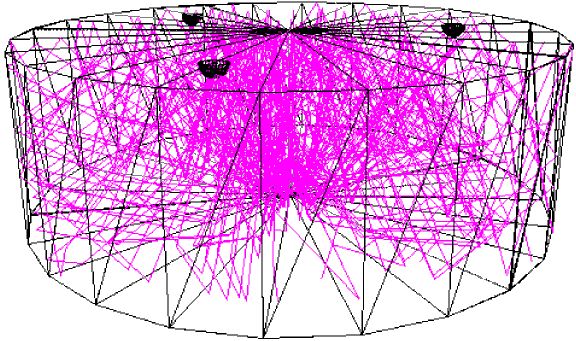
\includegraphics[width=0.7\textwidth]{fig/simulacionAuger/cher_tank_sim}
			\caption{Simulaci\'on de fotones Cherenkov generados en el pasaje de un electron de baja energ\'ia a trav\'es del tanque.}
			\label{fig:cher_tank_sim}
			\end{center}
		\end{figure}
		%
		
		Adem\'as de toda la f\'isica involucrada, la electr\'onica de la estaci\'on tambien es simulada.
		Luego de esta etapa, cada tanque involucrado en un evento tiene sus trazas FADC calculadas listas para ser analizadas por los algoritmos de trigger.
		
		\subsubsection{Trigger}
		
		Una vez que las trazas FADC fueron calculadas, \Offline{} posee algoritmos que calculan cada nivel de trigger del detector, desde disparos locales T2 hasta CDAS T4 y T5, especificados en la secci\'on \ref{sbsc:trig_levels}.
		

	\section{Almacenamiento y manejo de los datos}
	
	En la realización de este trabajo se hacen miles de simulaciones que sumándolas requieren mucho tiempo de cálculo.
	Además, la salida de estas miles de simulaciones debe ser guardada y el espacio en disco se vuelve muchas veces un problema.
	
	Para poder resolver esta problemática se hace uso del centro de cálculo CC-IN2P3 que responde a las necesidades en recursos informáticos de físicos que trabajan en 3 grandes temas de la física:
	
	\begin{itemize}
	\item Física de Partículas
	\item Física Nuclear
	\item Astrofísica, dentro de las cuales se encuentra el proyecto Observatorio Pierre Auger
	\end{itemize}
	
	El Centro de Cálculo de la IN2P3 está compuesto de materiales heterogéneos que se reparten en 4 grandes categorías:
	
	\begin{itemize}
	\item Plataforma de cálculo.
	\item Bandas magnéticas para guardar información.
	\item Discos para guardar información.
	\item Servidores que permiten la comunicación de las tres áreas anteriores.
	\end{itemize}
	
	{\bf Plataforma de cálculo:} tiene un poder de cálculo de más de 11 millones de SpecInt2000 (25,7 Teraflops).
	El sistema que se utiliza para administrar esta plataforma es Scientific Linux.
	Es esta plataforma la que se encarga de realizar todos los cálculos necesarios para las simulaciones según se especifique.
	
	{\bf Bandas magnéticas para guardar información:} Se dispone de dos lectoras de bandas magnéticas que tienen una capacidad de \cant{7}{PB}=\cant{7\ 10^6}{GB}.
	Esto básicamente permite almacenar toda la información que sea necesaria.
	El problema de la banda magnética consiste en la velocidad de acceso y en las dificultades que presenta cuando quieren acceder muchos usuarios en simultaneo.
	
	{\bf Discos para guardar información:} Para resolver los problemas de la banda magnética, se otorga a cada usuario un espacio de disco del orden del GigaByte que se utiliza para tener los archivos que necesiten actualización frecuente. 
	Este espacio juega el rol de {\em cache}.
	
	\section{An\'alisis de datos}
	
	Para la implementación de los programas de análisis de datos se seleccionó al lenguaje de programación C++. Existen varias razones para utilizar este lenguaje orientado a objetos, a saber:
	
	\begin{itemize}
	\item Los proyectos grandes, con muchas personas desarroll\'andolo en paralelo, son mucho m\'as f\'aciles de coordinar cuando se utiliza C++ que cuando se utiliza FORTRAN o C.
	\item Existe actualmente una gran comunidad que utiliza C++, proveyendo herramientas, soporte y utilidades.
	\item Es m\'as probable que las personas j\'ovenes de la colaboraci\'on est\'en familiarizados con C++ que con FORTRAN.
	\end{itemize}

	Una de las herramientas m\'as utilizada en la colaboraci\'on son las librer\'ias de ROOT \cite{ROOT} desarrolladas por el CERN.
	Estas constan de un enorme conjunto de herramientas que facilitan la implementación de programas de análisis de datos. 
	Entre otras cosas, incluye tanto herramientas de minimización (muy útiles en la realización de ajustes) como de visualización y lectura/escritura de grandes volúmenes de datos.